\documentclass[11pt]{article}
\usepackage[textwidth=18.0cm, textheight=23.0cm, top=2.0cm]{geometry}
\usepackage{pst-all}
\usepackage{amssymb}
\usepackage{tikz}
\usepackage{underscore}\begin{document}
\pagestyle{empty}


ClassName: \underline{\textbf{Class_10.2bp-30}}
\par
BinSize: \underline{\textbf{100 × 100}}
\par
ReduceSize: \underline{\textbf{100 × 100}}
\par
TypeNum: \underline{\textbf{80}}
\par
Num: \underline{\textbf{80}}
\par
OutS: \underline{\textbf{130000}}
\par
InS: \underline{\textbf{117391}}
\par
Rate: \underline{\textbf{0.903}}
\par
UB: \underline{\textbf{13}}
\par
LB0: \underline{\textbf{12}}
\par
LB: \underline{\textbf{13}}
\par
LBWithCut: \underline{\textbf{13}}
\par
NodeCut: \underline{\textbf{0}}
\par
ExtendedNodeCnt: \underline{\textbf{1}}
\par
GenNodeCnt: \underline{\textbf{1}}
\par
PrimalNode: \underline{\textbf{0}}
\par
ColumnCount: \underline{\textbf{77}}
\par
TotalCutCount: \underline{\textbf{0}}
\par
RootCutCount: \underline{\textbf{0}}
\par
LPSolverCnt: \underline{\textbf{64}}
\par
PricingSolverCnt: \underline{\textbf{64}}
\par
BranchAndBoundNum: \underline{\textbf{1}}
\par
isOpt: \underline{\textbf{false}}
\par
TimeOnPrimal: \underline{\textbf{0.000 s}}
\par
TimeOnPricing: \underline{\textbf{3600.020 s}}
\par
TimeOnRmp: \underline{\textbf{0.129 s}}
\par
TotalTime: \underline{\textbf{3600.213 s}}
\par
\newpage


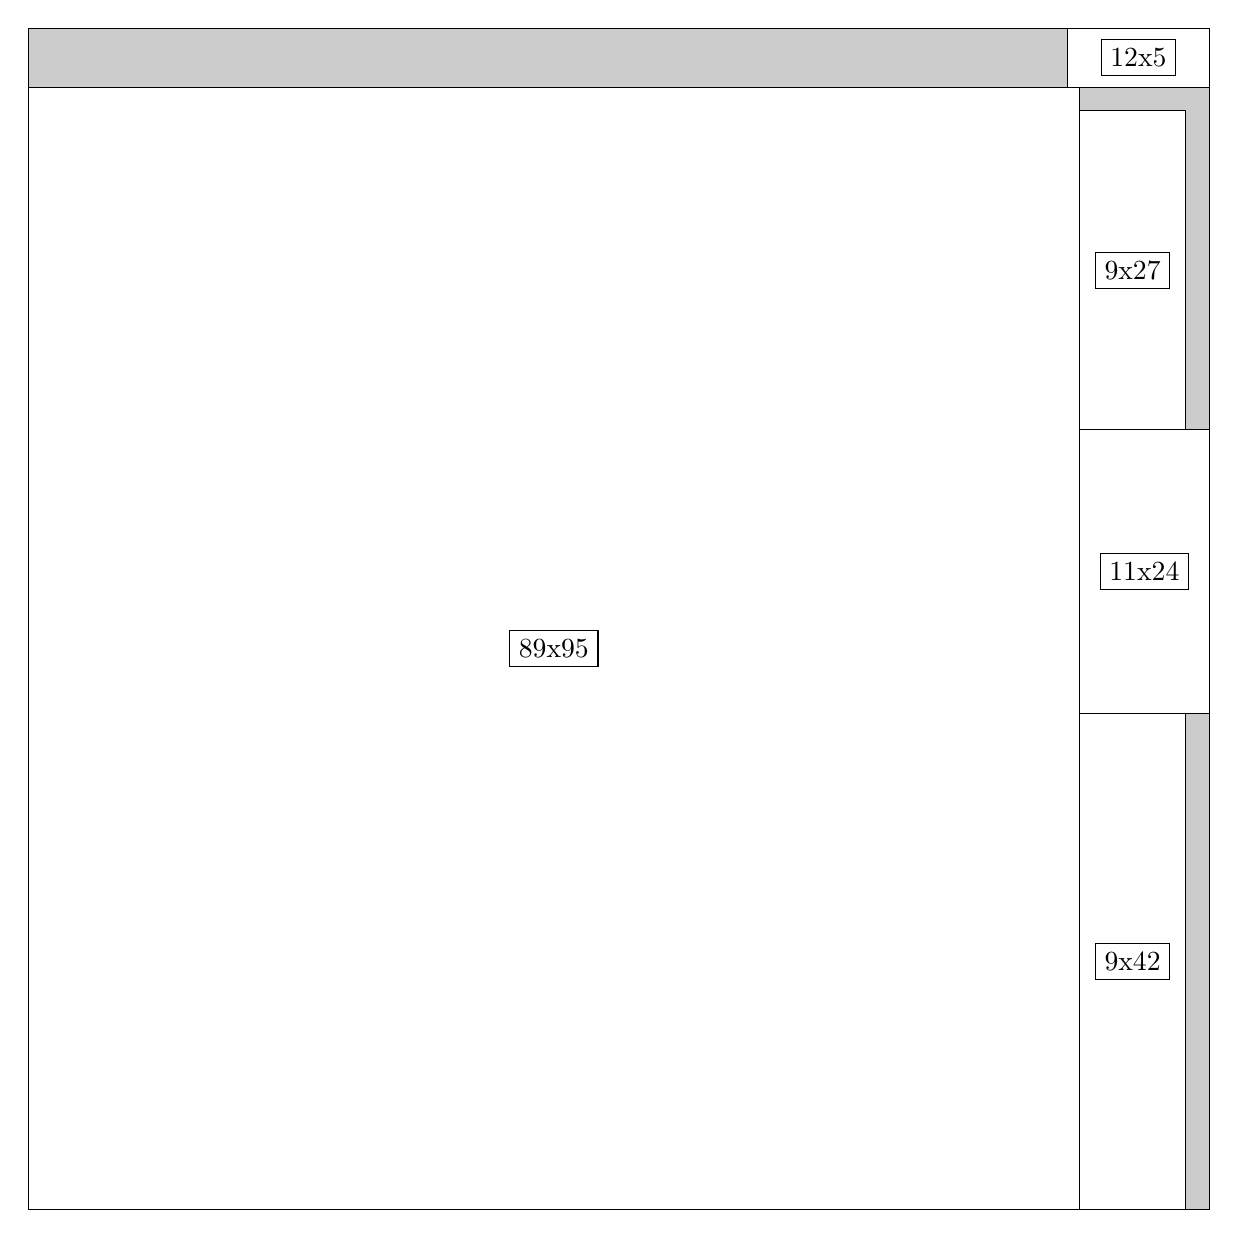
\begin{tikzpicture}[shorten >=1pt,scale=1.0,every node/.style={scale=1.0},->]
\tikzstyle{vertex}=[circle,fill=black!25,minimum size=14pt,inner sep=0pt]
\filldraw[fill=gray!40!white, draw=black] (0,0) rectangle (15.0,15.0);
\foreach \name/\x/\y/\w/\h in {89x95/0.0/0.0/13.35/14.25,9x42/13.35/0.0/1.3499999999999999/6.3,11x24/13.35/6.3/1.65/3.5999999999999996,9x27/13.35/9.9/1.3499999999999999/4.05,12x5/13.2/14.25/1.7999999999999998/0.75}
\filldraw[fill=white!40!white, draw=black] (\x,\y) rectangle node[draw] (\name) {\name} ++(\w,\h);
\end{tikzpicture}


w =89 , h =95 , x =0 , y =0 , v =8455
\par
w =9 , h =42 , x =89 , y =0 , v =378
\par
w =11 , h =24 , x =89 , y =42 , v =264
\par
w =9 , h =27 , x =89 , y =66 , v =243
\par
w =12 , h =5 , x =88 , y =95 , v =60
\par
\newpage


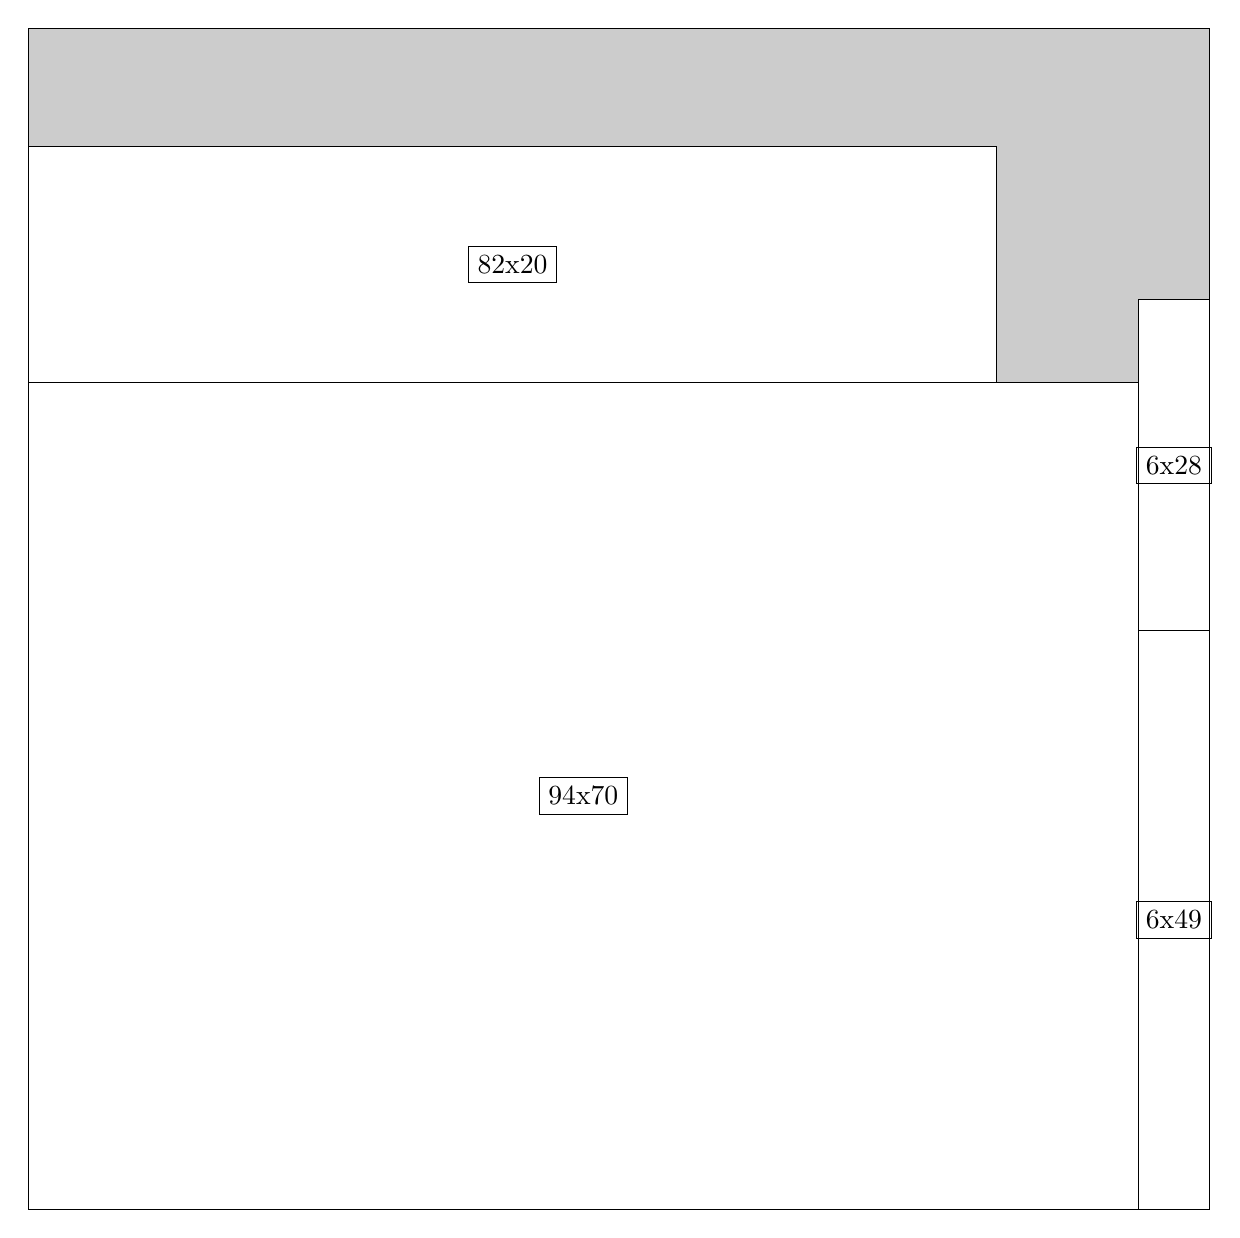
\begin{tikzpicture}[shorten >=1pt,scale=1.0,every node/.style={scale=1.0},->]
\tikzstyle{vertex}=[circle,fill=black!25,minimum size=14pt,inner sep=0pt]
\filldraw[fill=gray!40!white, draw=black] (0,0) rectangle (15.0,15.0);
\foreach \name/\x/\y/\w/\h in {94x70/0.0/0.0/14.1/10.5,82x20/0.0/10.5/12.299999999999999/3.0,6x49/14.1/0.0/0.8999999999999999/7.35,6x28/14.1/7.35/0.8999999999999999/4.2}
\filldraw[fill=white!40!white, draw=black] (\x,\y) rectangle node[draw] (\name) {\name} ++(\w,\h);
\end{tikzpicture}


w =94 , h =70 , x =0 , y =0 , v =6580
\par
w =82 , h =20 , x =0 , y =70 , v =1640
\par
w =6 , h =49 , x =94 , y =0 , v =294
\par
w =6 , h =28 , x =94 , y =49 , v =168
\par
\newpage


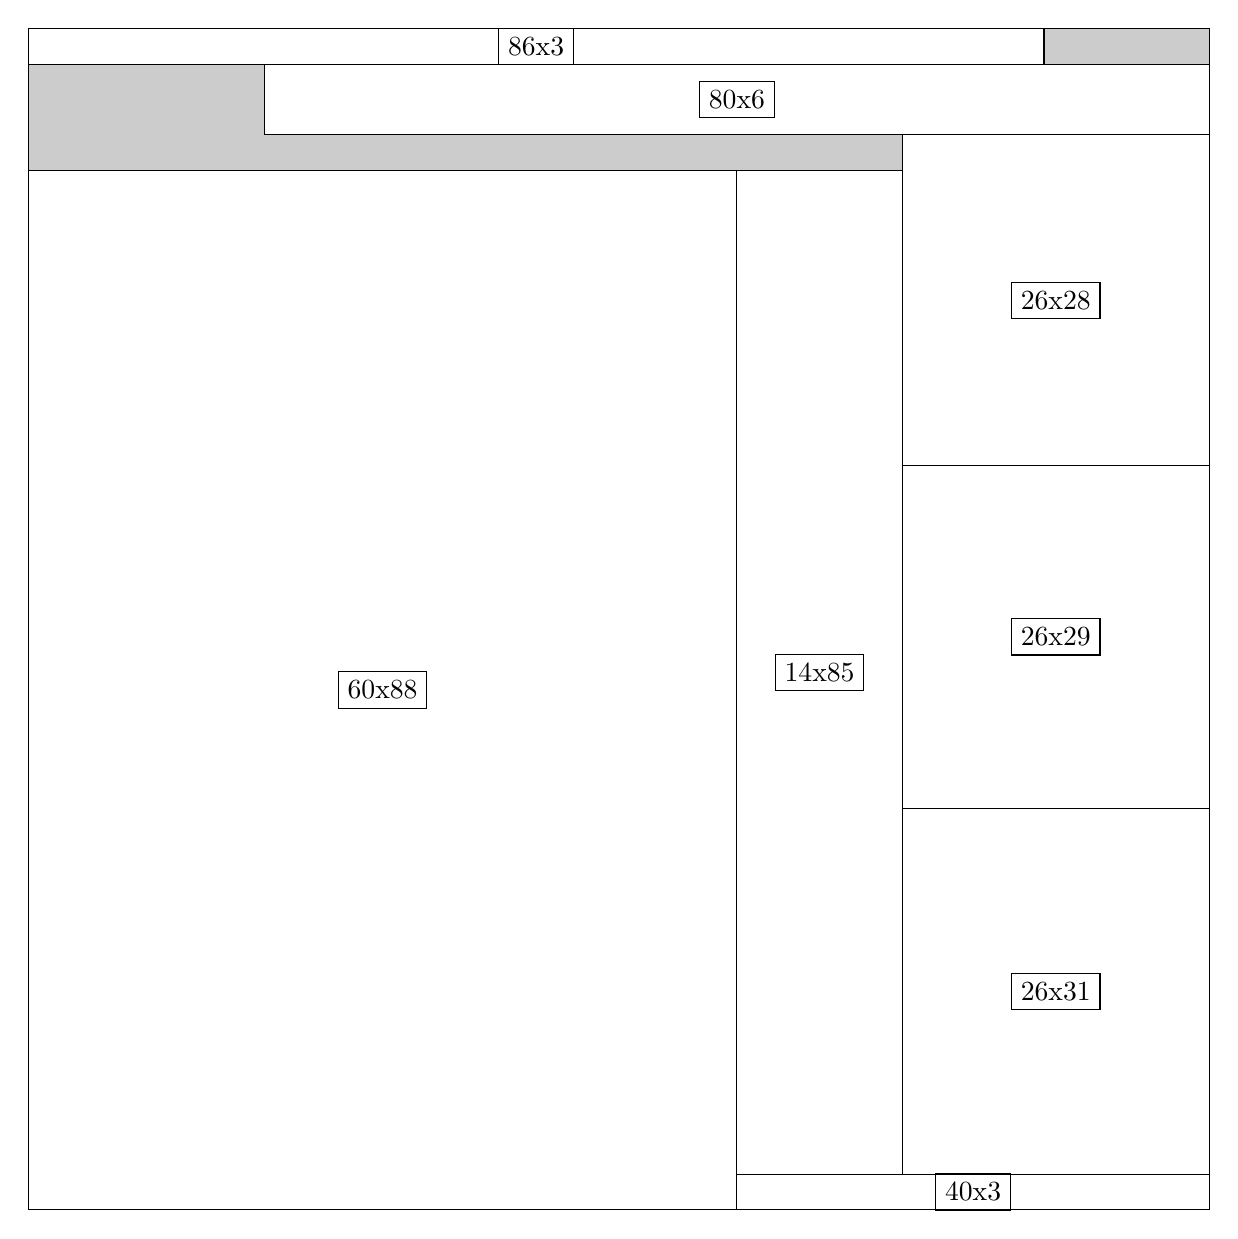
\begin{tikzpicture}[shorten >=1pt,scale=1.0,every node/.style={scale=1.0},->]
\tikzstyle{vertex}=[circle,fill=black!25,minimum size=14pt,inner sep=0pt]
\filldraw[fill=gray!40!white, draw=black] (0,0) rectangle (15.0,15.0);
\foreach \name/\x/\y/\w/\h in {60x88/0.0/0.0/9.0/13.2,14x85/9.0/0.44999999999999996/2.1/12.75,26x31/11.1/0.44999999999999996/3.9/4.6499999999999995,26x29/11.1/5.1/3.9/4.35,26x28/11.1/9.45/3.9/4.2,80x6/3.0/13.65/12.0/0.8999999999999999,86x3/0.0/14.549999999999999/12.9/0.44999999999999996,40x3/9.0/0.0/6.0/0.44999999999999996}
\filldraw[fill=white!40!white, draw=black] (\x,\y) rectangle node[draw] (\name) {\name} ++(\w,\h);
\end{tikzpicture}


w =60 , h =88 , x =0 , y =0 , v =5280
\par
w =14 , h =85 , x =60 , y =3 , v =1190
\par
w =26 , h =31 , x =74 , y =3 , v =806
\par
w =26 , h =29 , x =74 , y =34 , v =754
\par
w =26 , h =28 , x =74 , y =63 , v =728
\par
w =80 , h =6 , x =20 , y =91 , v =480
\par
w =86 , h =3 , x =0 , y =97 , v =258
\par
w =40 , h =3 , x =60 , y =0 , v =120
\par
\newpage


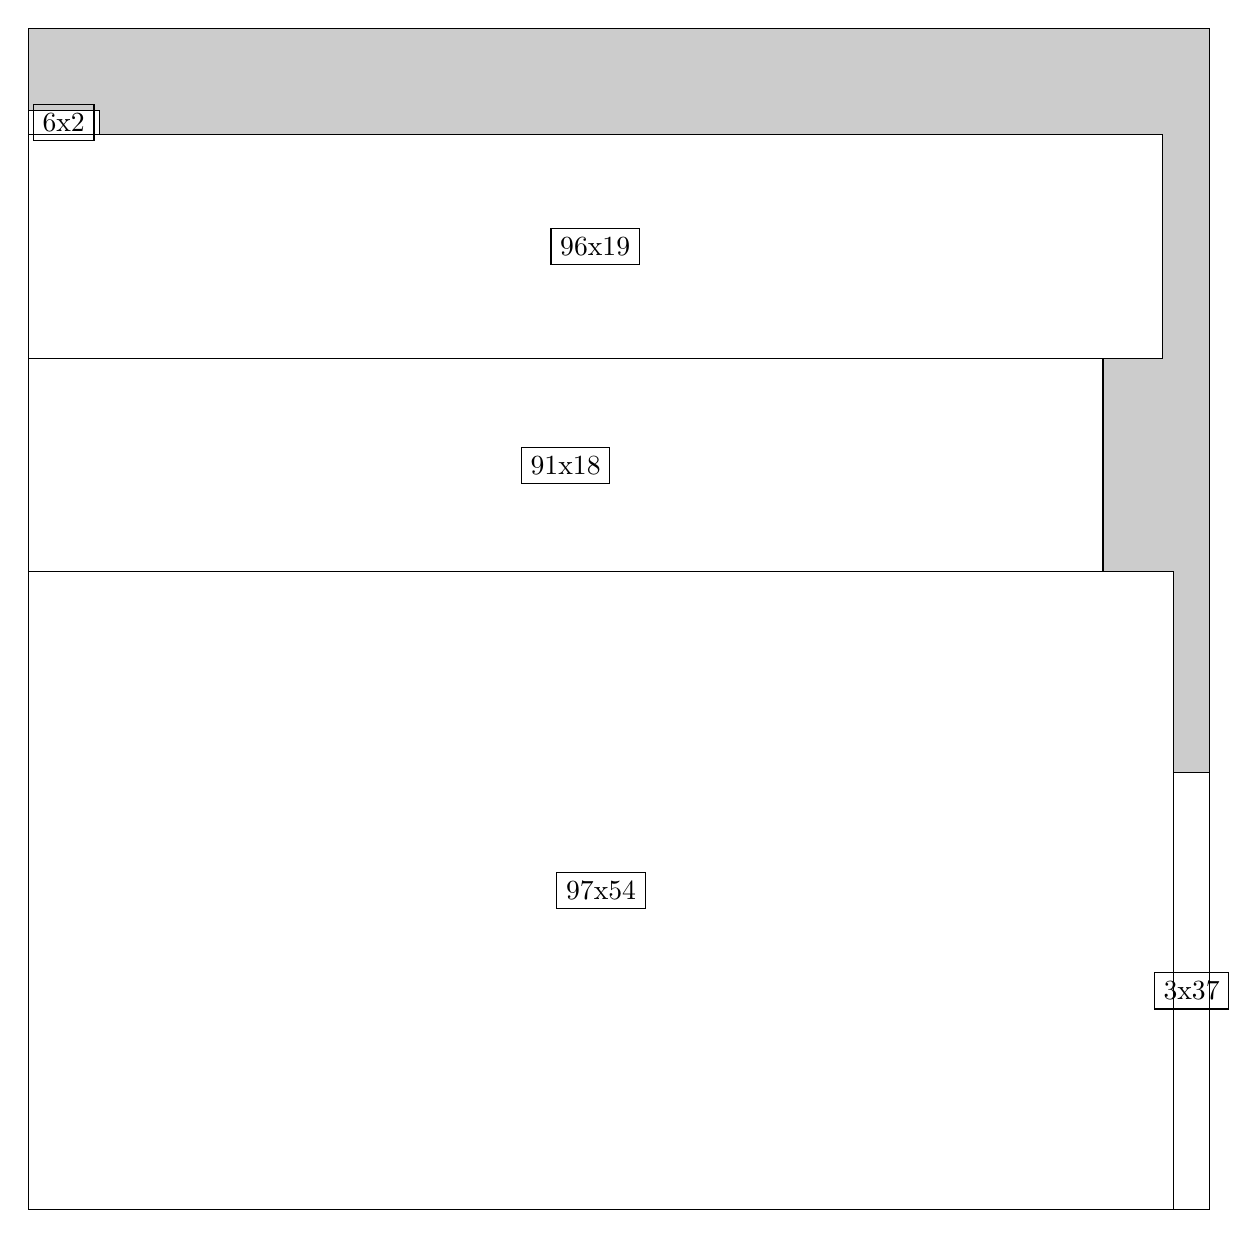
\begin{tikzpicture}[shorten >=1pt,scale=1.0,every node/.style={scale=1.0},->]
\tikzstyle{vertex}=[circle,fill=black!25,minimum size=14pt,inner sep=0pt]
\filldraw[fill=gray!40!white, draw=black] (0,0) rectangle (15.0,15.0);
\foreach \name/\x/\y/\w/\h in {97x54/0.0/0.0/14.549999999999999/8.1,96x19/0.0/10.799999999999999/14.399999999999999/2.85,91x18/0.0/8.1/13.65/2.6999999999999997,3x37/14.549999999999999/0.0/0.44999999999999996/5.55,6x2/0.0/13.65/0.8999999999999999/0.3}
\filldraw[fill=white!40!white, draw=black] (\x,\y) rectangle node[draw] (\name) {\name} ++(\w,\h);
\end{tikzpicture}


w =97 , h =54 , x =0 , y =0 , v =5238
\par
w =96 , h =19 , x =0 , y =72 , v =1824
\par
w =91 , h =18 , x =0 , y =54 , v =1638
\par
w =3 , h =37 , x =97 , y =0 , v =111
\par
w =6 , h =2 , x =0 , y =91 , v =12
\par
\newpage


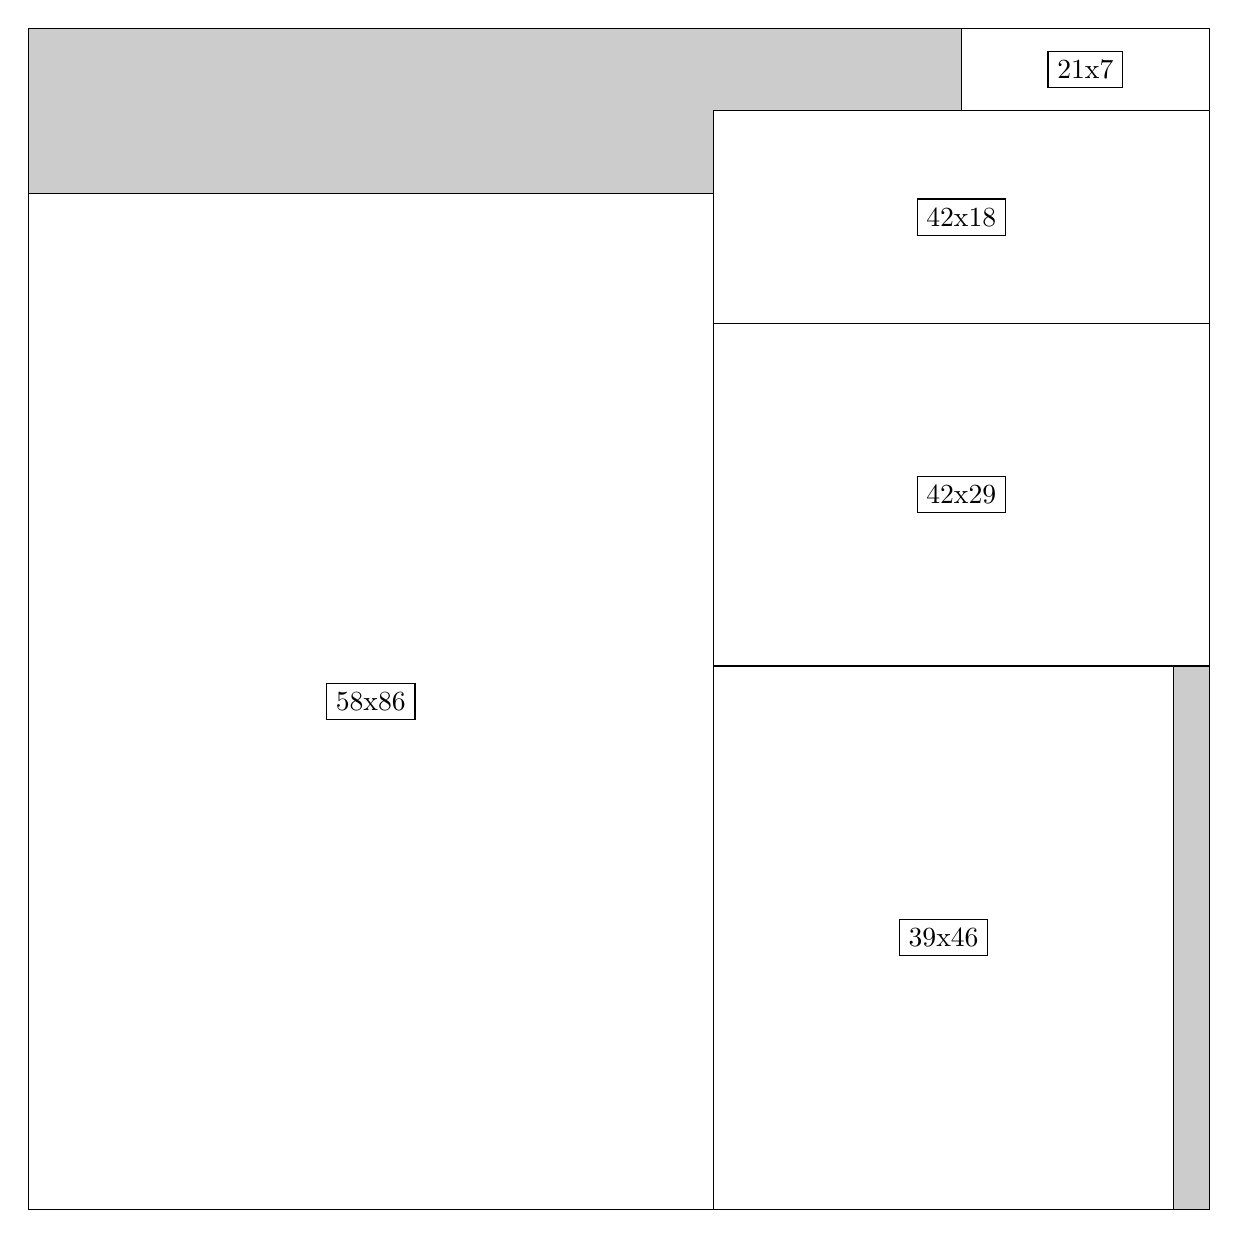
\begin{tikzpicture}[shorten >=1pt,scale=1.0,every node/.style={scale=1.0},->]
\tikzstyle{vertex}=[circle,fill=black!25,minimum size=14pt,inner sep=0pt]
\filldraw[fill=gray!40!white, draw=black] (0,0) rectangle (15.0,15.0);
\foreach \name/\x/\y/\w/\h in {39x46/8.7/0.0/5.85/6.8999999999999995,58x86/0.0/0.0/8.7/12.9,42x29/8.7/6.8999999999999995/6.3/4.35,42x18/8.7/11.25/6.3/2.6999999999999997,21x7/11.85/13.95/3.15/1.05}
\filldraw[fill=white!40!white, draw=black] (\x,\y) rectangle node[draw] (\name) {\name} ++(\w,\h);
\end{tikzpicture}


w =39 , h =46 , x =58 , y =0 , v =1794
\par
w =58 , h =86 , x =0 , y =0 , v =4988
\par
w =42 , h =29 , x =58 , y =46 , v =1218
\par
w =42 , h =18 , x =58 , y =75 , v =756
\par
w =21 , h =7 , x =79 , y =93 , v =147
\par
\newpage


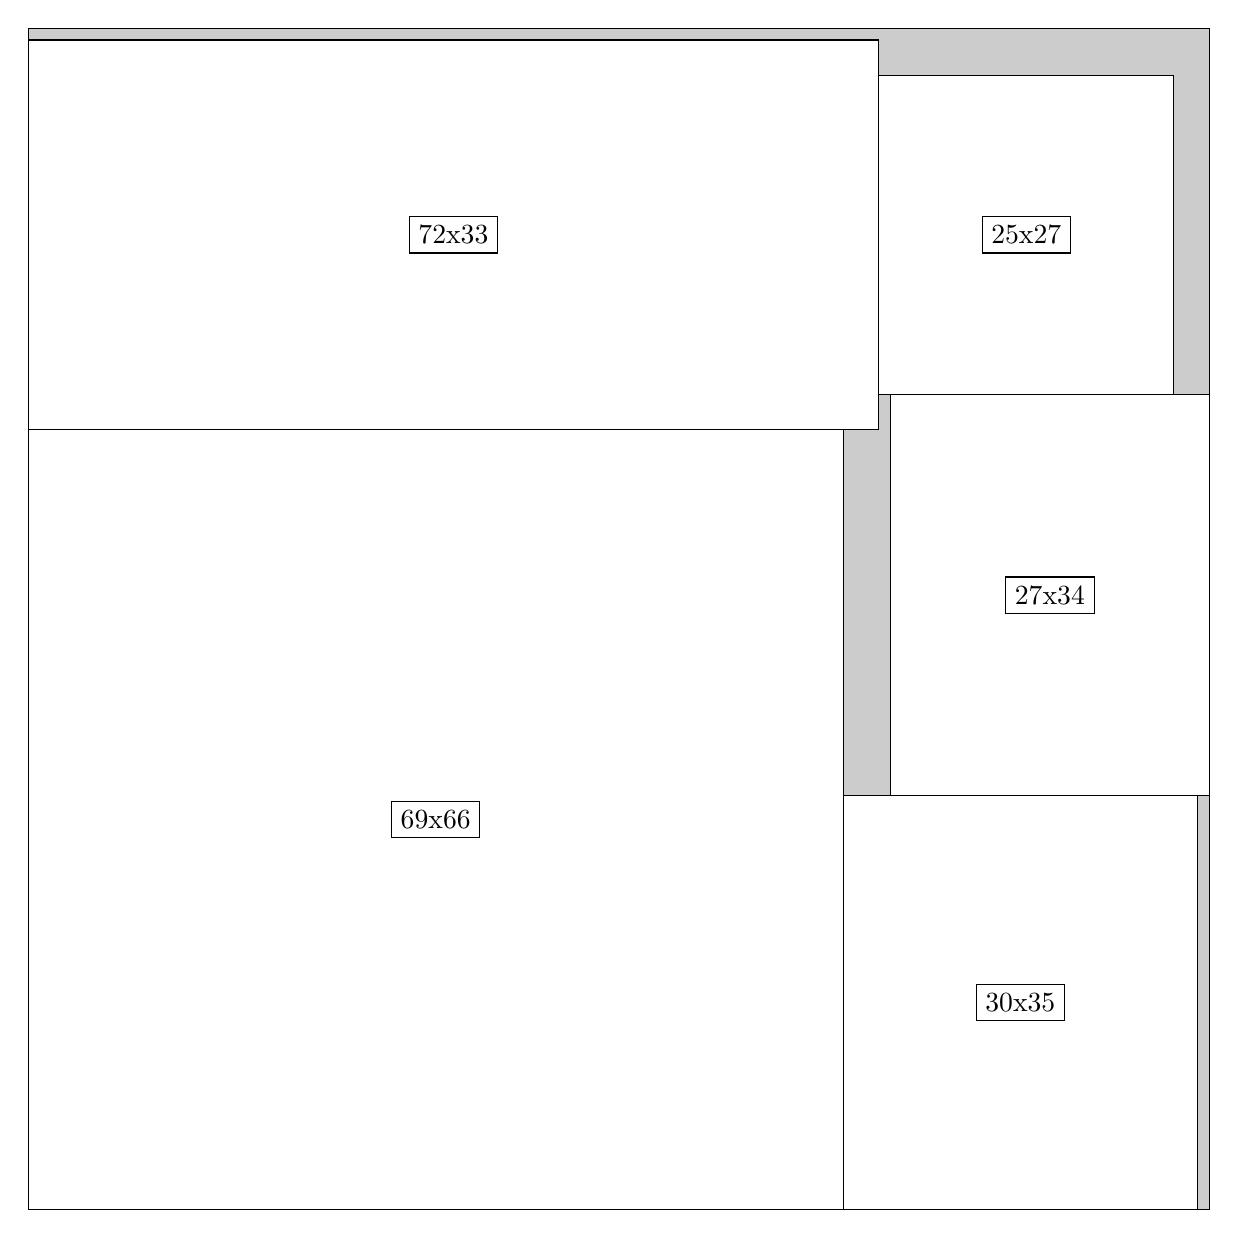
\begin{tikzpicture}[shorten >=1pt,scale=1.0,every node/.style={scale=1.0},->]
\tikzstyle{vertex}=[circle,fill=black!25,minimum size=14pt,inner sep=0pt]
\filldraw[fill=gray!40!white, draw=black] (0,0) rectangle (15.0,15.0);
\foreach \name/\x/\y/\w/\h in {69x66/0.0/0.0/10.35/9.9,72x33/0.0/9.9/10.799999999999999/4.95,30x35/10.35/0.0/4.5/5.25,27x34/10.95/5.25/4.05/5.1,25x27/10.799999999999999/10.35/3.75/4.05}
\filldraw[fill=white!40!white, draw=black] (\x,\y) rectangle node[draw] (\name) {\name} ++(\w,\h);
\end{tikzpicture}


w =69 , h =66 , x =0 , y =0 , v =4554
\par
w =72 , h =33 , x =0 , y =66 , v =2376
\par
w =30 , h =35 , x =69 , y =0 , v =1050
\par
w =27 , h =34 , x =73 , y =35 , v =918
\par
w =25 , h =27 , x =72 , y =69 , v =675
\par
\newpage


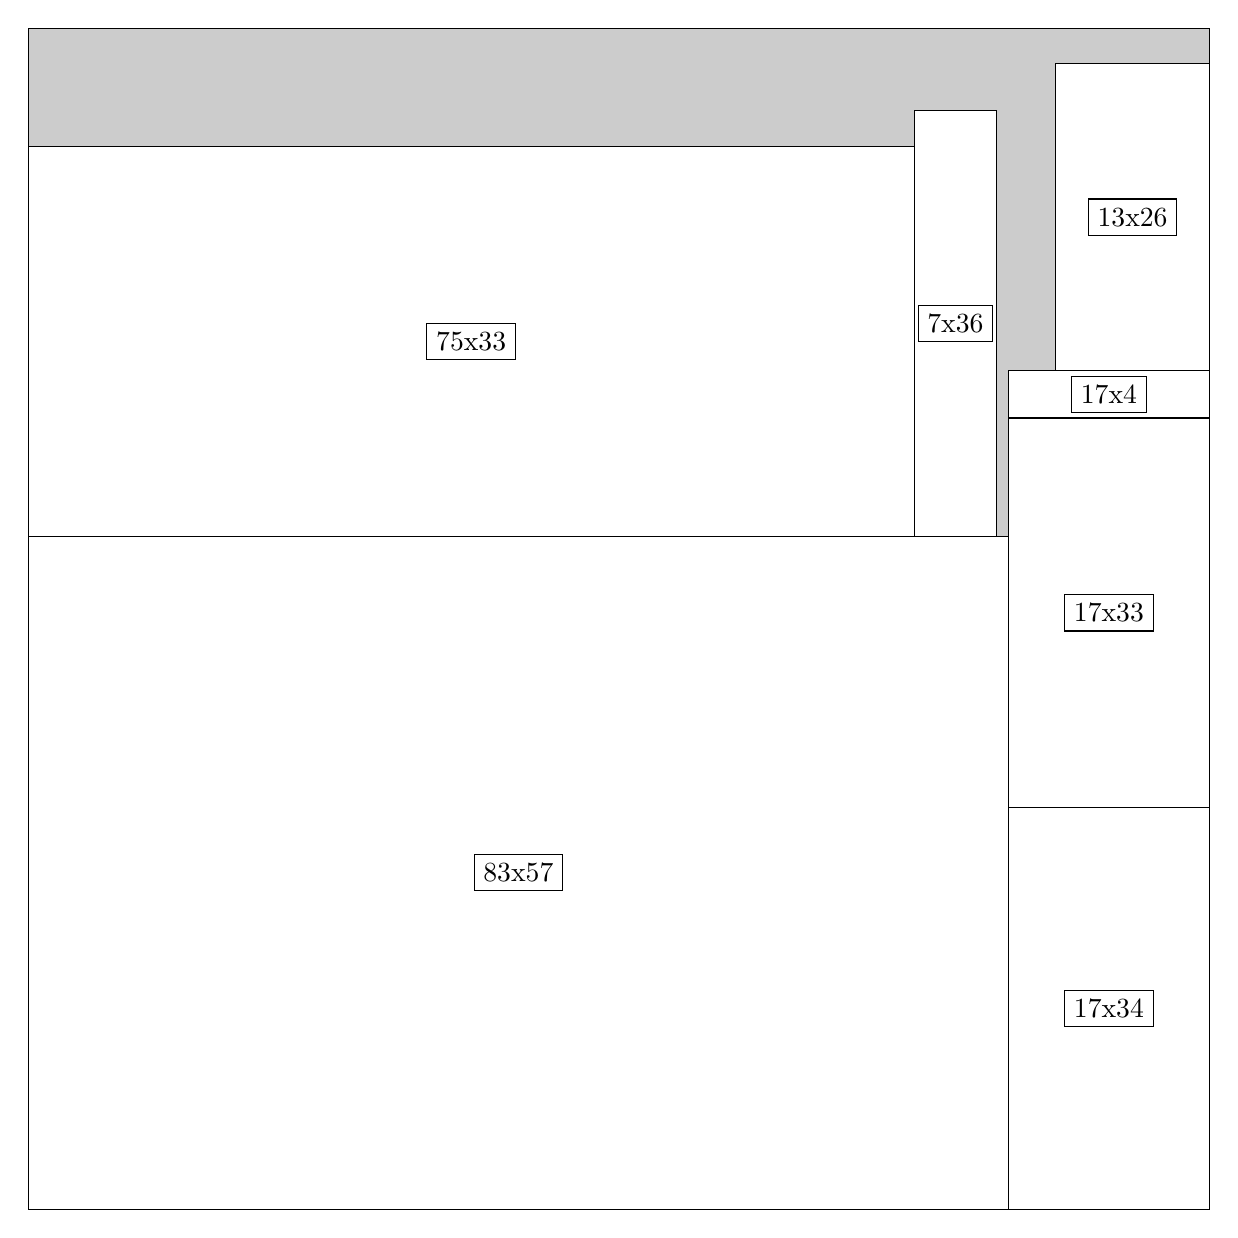
\begin{tikzpicture}[shorten >=1pt,scale=1.0,every node/.style={scale=1.0},->]
\tikzstyle{vertex}=[circle,fill=black!25,minimum size=14pt,inner sep=0pt]
\filldraw[fill=gray!40!white, draw=black] (0,0) rectangle (15.0,15.0);
\foreach \name/\x/\y/\w/\h in {83x57/0.0/0.0/12.45/8.549999999999999,75x33/0.0/8.549999999999999/11.25/4.95,17x34/12.45/0.0/2.55/5.1,17x33/12.45/5.1/2.55/4.95,13x26/13.049999999999999/10.65/1.95/3.9,7x36/11.25/8.549999999999999/1.05/5.3999999999999995,17x4/12.45/10.049999999999999/2.55/0.6}
\filldraw[fill=white!40!white, draw=black] (\x,\y) rectangle node[draw] (\name) {\name} ++(\w,\h);
\end{tikzpicture}


w =83 , h =57 , x =0 , y =0 , v =4731
\par
w =75 , h =33 , x =0 , y =57 , v =2475
\par
w =17 , h =34 , x =83 , y =0 , v =578
\par
w =17 , h =33 , x =83 , y =34 , v =561
\par
w =13 , h =26 , x =87 , y =71 , v =338
\par
w =7 , h =36 , x =75 , y =57 , v =252
\par
w =17 , h =4 , x =83 , y =67 , v =68
\par
\newpage


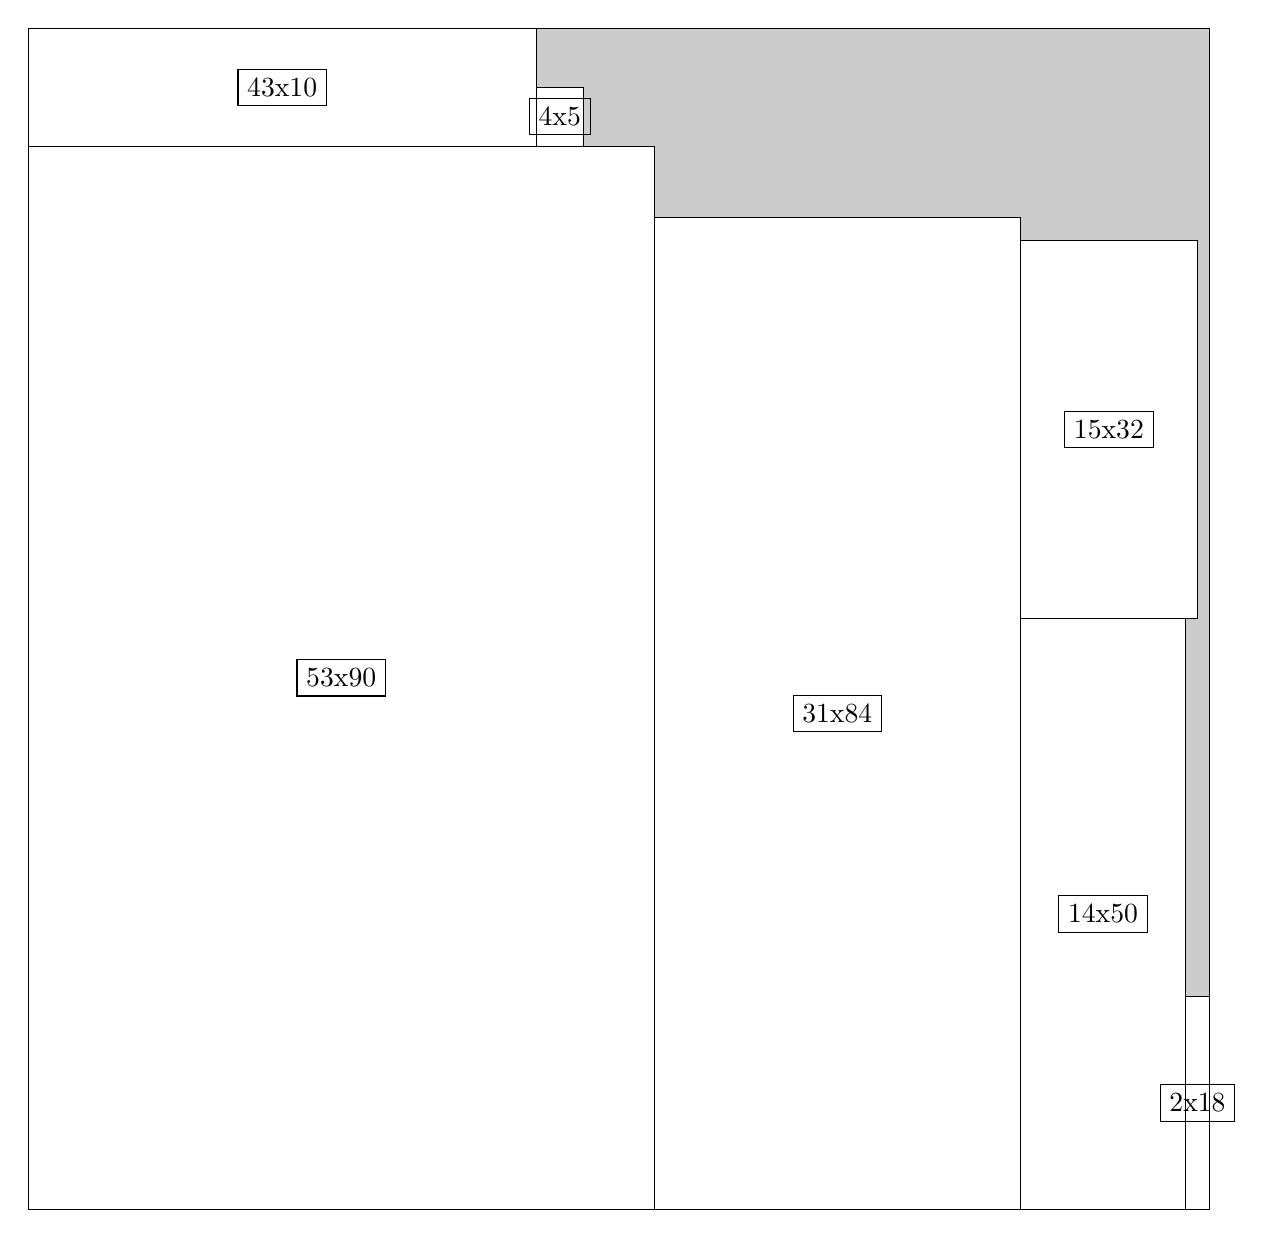
\begin{tikzpicture}[shorten >=1pt,scale=1.0,every node/.style={scale=1.0},->]
\tikzstyle{vertex}=[circle,fill=black!25,minimum size=14pt,inner sep=0pt]
\filldraw[fill=gray!40!white, draw=black] (0,0) rectangle (15.0,15.0);
\foreach \name/\x/\y/\w/\h in {53x90/0.0/0.0/7.949999999999999/13.5,31x84/7.949999999999999/0.0/4.6499999999999995/12.6,14x50/12.6/0.0/2.1/7.5,15x32/12.6/7.5/2.25/4.8,43x10/0.0/13.5/6.45/1.5,2x18/14.7/0.0/0.3/2.6999999999999997,4x5/6.45/13.5/0.6/0.75}
\filldraw[fill=white!40!white, draw=black] (\x,\y) rectangle node[draw] (\name) {\name} ++(\w,\h);
\end{tikzpicture}


w =53 , h =90 , x =0 , y =0 , v =4770
\par
w =31 , h =84 , x =53 , y =0 , v =2604
\par
w =14 , h =50 , x =84 , y =0 , v =700
\par
w =15 , h =32 , x =84 , y =50 , v =480
\par
w =43 , h =10 , x =0 , y =90 , v =430
\par
w =2 , h =18 , x =98 , y =0 , v =36
\par
w =4 , h =5 , x =43 , y =90 , v =20
\par
\newpage


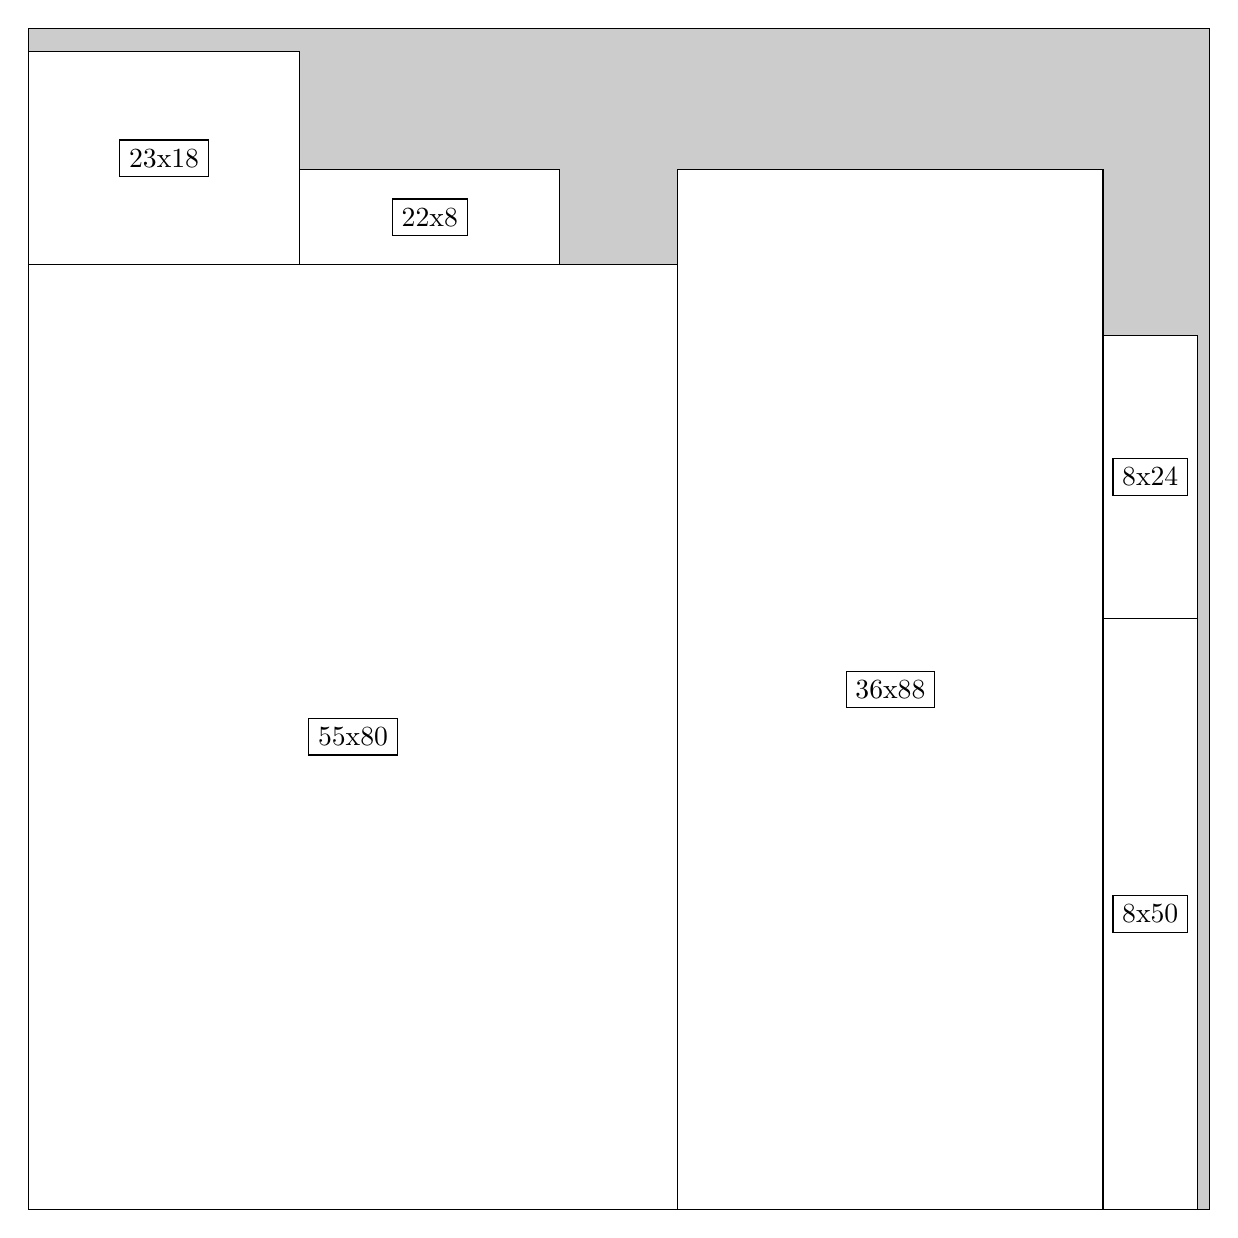
\begin{tikzpicture}[shorten >=1pt,scale=1.0,every node/.style={scale=1.0},->]
\tikzstyle{vertex}=[circle,fill=black!25,minimum size=14pt,inner sep=0pt]
\filldraw[fill=gray!40!white, draw=black] (0,0) rectangle (15.0,15.0);
\foreach \name/\x/\y/\w/\h in {55x80/0.0/0.0/8.25/12.0,36x88/8.25/0.0/5.3999999999999995/13.2,23x18/0.0/12.0/3.4499999999999997/2.6999999999999997,8x50/13.65/0.0/1.2/7.5,8x24/13.65/7.5/1.2/3.5999999999999996,22x8/3.4499999999999997/12.0/3.3/1.2}
\filldraw[fill=white!40!white, draw=black] (\x,\y) rectangle node[draw] (\name) {\name} ++(\w,\h);
\end{tikzpicture}


w =55 , h =80 , x =0 , y =0 , v =4400
\par
w =36 , h =88 , x =55 , y =0 , v =3168
\par
w =23 , h =18 , x =0 , y =80 , v =414
\par
w =8 , h =50 , x =91 , y =0 , v =400
\par
w =8 , h =24 , x =91 , y =50 , v =192
\par
w =22 , h =8 , x =23 , y =80 , v =176
\par
\newpage


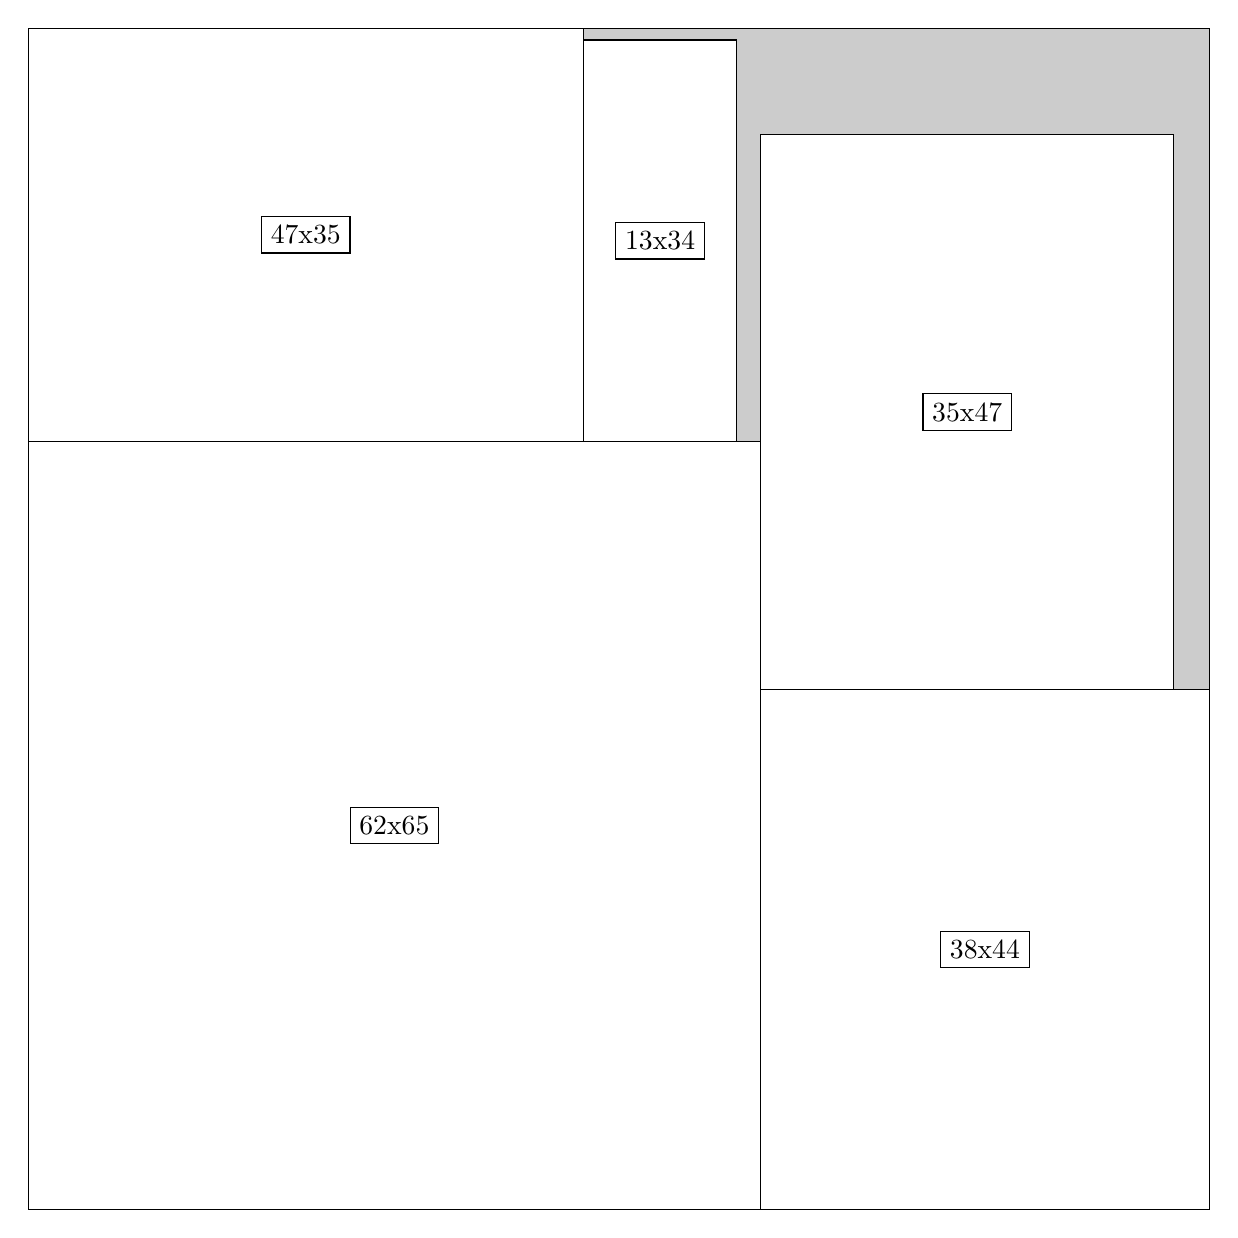
\begin{tikzpicture}[shorten >=1pt,scale=1.0,every node/.style={scale=1.0},->]
\tikzstyle{vertex}=[circle,fill=black!25,minimum size=14pt,inner sep=0pt]
\filldraw[fill=gray!40!white, draw=black] (0,0) rectangle (15.0,15.0);
\foreach \name/\x/\y/\w/\h in {62x65/0.0/0.0/9.299999999999999/9.75,38x44/9.299999999999999/0.0/5.7/6.6,47x35/0.0/9.75/7.05/5.25,35x47/9.299999999999999/6.6/5.25/7.05,13x34/7.05/9.75/1.95/5.1}
\filldraw[fill=white!40!white, draw=black] (\x,\y) rectangle node[draw] (\name) {\name} ++(\w,\h);
\end{tikzpicture}


w =62 , h =65 , x =0 , y =0 , v =4030
\par
w =38 , h =44 , x =62 , y =0 , v =1672
\par
w =47 , h =35 , x =0 , y =65 , v =1645
\par
w =35 , h =47 , x =62 , y =44 , v =1645
\par
w =13 , h =34 , x =47 , y =65 , v =442
\par
\newpage


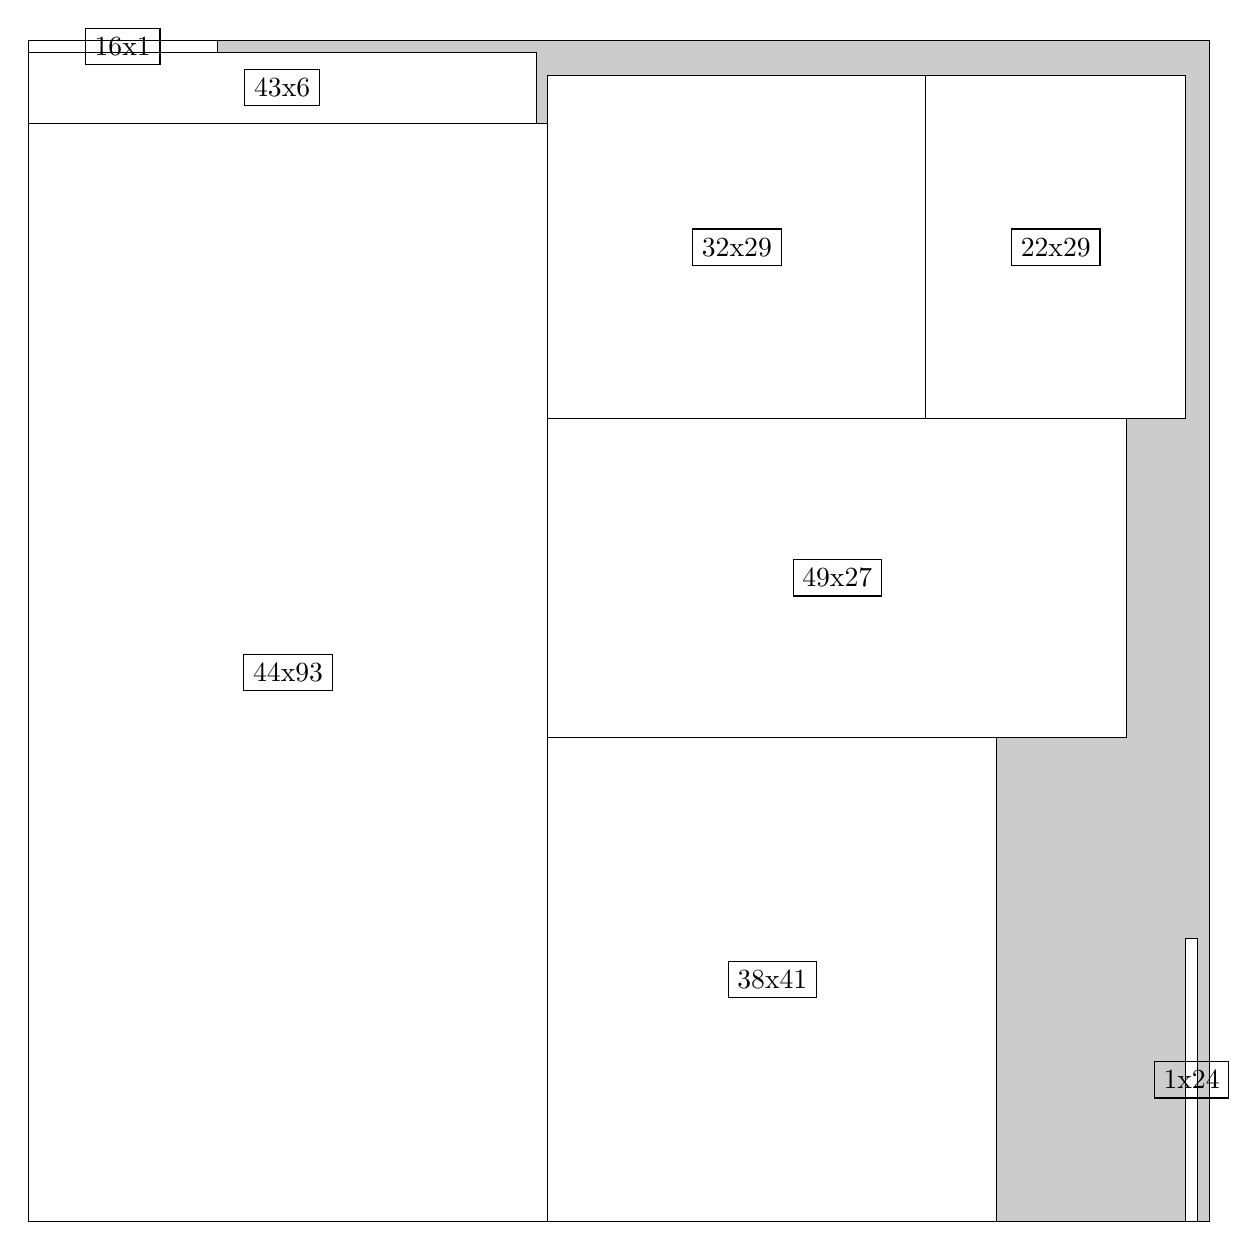
\begin{tikzpicture}[shorten >=1pt,scale=1.0,every node/.style={scale=1.0},->]
\tikzstyle{vertex}=[circle,fill=black!25,minimum size=14pt,inner sep=0pt]
\filldraw[fill=gray!40!white, draw=black] (0,0) rectangle (15.0,15.0);
\foreach \name/\x/\y/\w/\h in {44x93/0.0/0.0/6.6/13.95,38x41/6.6/0.0/5.7/6.1499999999999995,49x27/6.6/6.1499999999999995/7.35/4.05,32x29/6.6/10.2/4.8/4.35,22x29/11.4/10.2/3.3/4.35,43x6/0.0/13.95/6.45/0.8999999999999999,1x24/14.7/0.0/0.15/3.5999999999999996,16x1/0.0/14.85/2.4/0.15}
\filldraw[fill=white!40!white, draw=black] (\x,\y) rectangle node[draw] (\name) {\name} ++(\w,\h);
\end{tikzpicture}


w =44 , h =93 , x =0 , y =0 , v =4092
\par
w =38 , h =41 , x =44 , y =0 , v =1558
\par
w =49 , h =27 , x =44 , y =41 , v =1323
\par
w =32 , h =29 , x =44 , y =68 , v =928
\par
w =22 , h =29 , x =76 , y =68 , v =638
\par
w =43 , h =6 , x =0 , y =93 , v =258
\par
w =1 , h =24 , x =98 , y =0 , v =24
\par
w =16 , h =1 , x =0 , y =99 , v =16
\par
\newpage


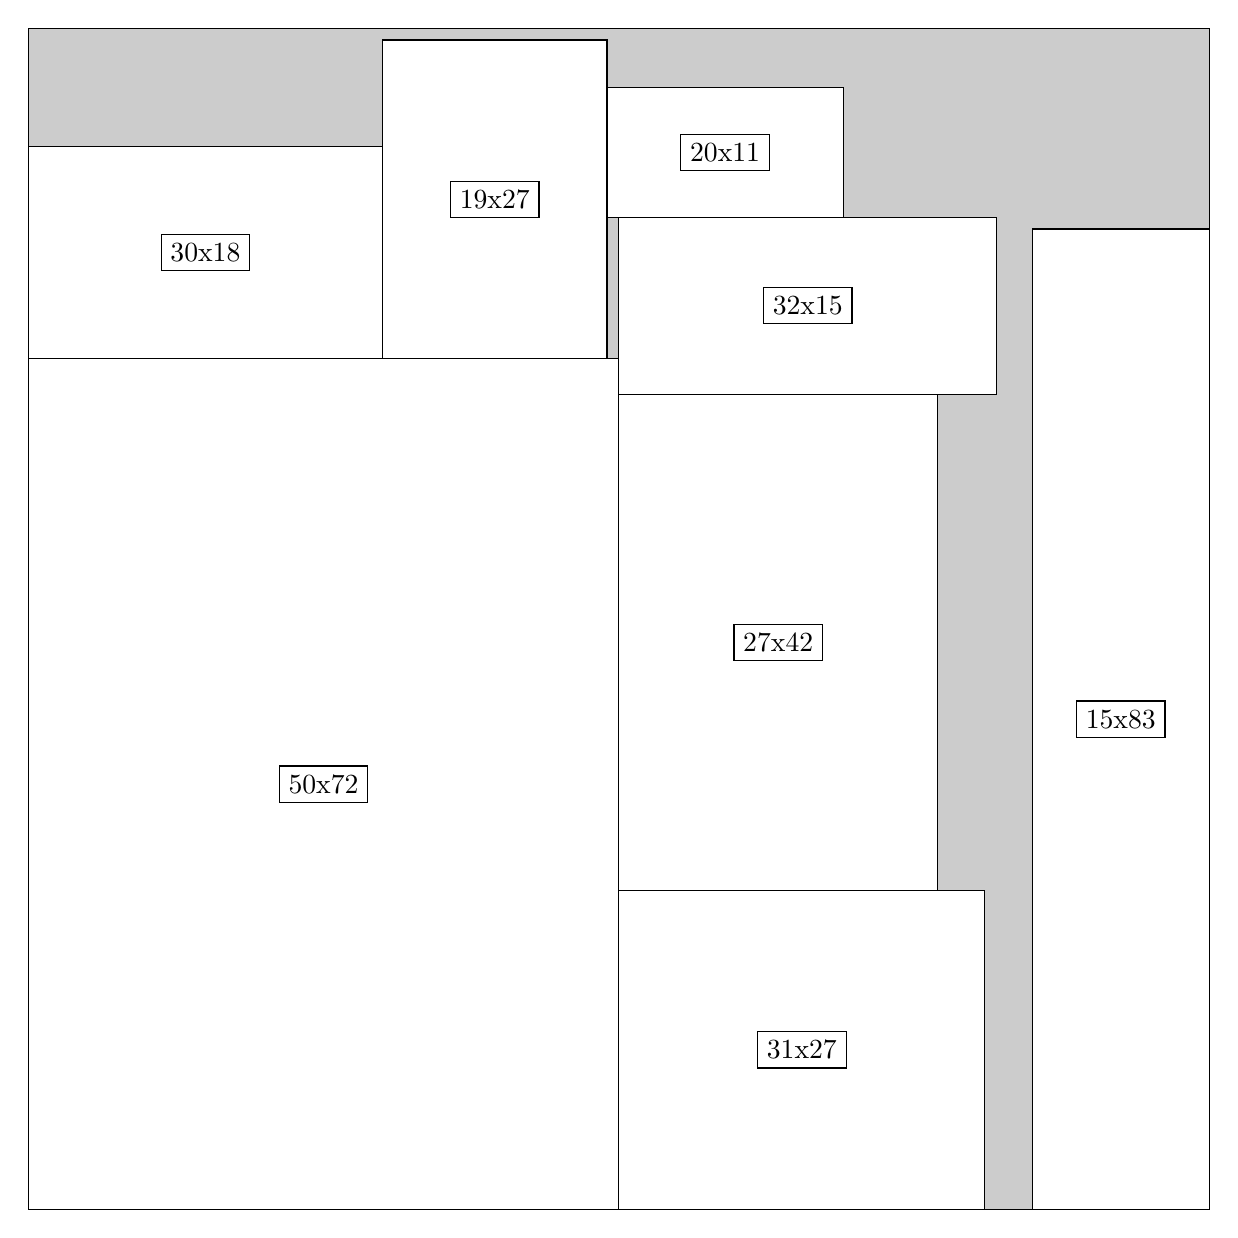
\begin{tikzpicture}[shorten >=1pt,scale=1.0,every node/.style={scale=1.0},->]
\tikzstyle{vertex}=[circle,fill=black!25,minimum size=14pt,inner sep=0pt]
\filldraw[fill=gray!40!white, draw=black] (0,0) rectangle (15.0,15.0);
\foreach \name/\x/\y/\w/\h in {50x72/0.0/0.0/7.5/10.799999999999999,31x27/7.5/0.0/4.6499999999999995/4.05,27x42/7.5/4.05/4.05/6.3,15x83/12.75/0.0/2.25/12.45,30x18/0.0/10.799999999999999/4.5/2.6999999999999997,19x27/4.5/10.799999999999999/2.85/4.05,32x15/7.5/10.35/4.8/2.25,20x11/7.35/12.6/3.0/1.65}
\filldraw[fill=white!40!white, draw=black] (\x,\y) rectangle node[draw] (\name) {\name} ++(\w,\h);
\end{tikzpicture}


w =50 , h =72 , x =0 , y =0 , v =3600
\par
w =31 , h =27 , x =50 , y =0 , v =837
\par
w =27 , h =42 , x =50 , y =27 , v =1134
\par
w =15 , h =83 , x =85 , y =0 , v =1245
\par
w =30 , h =18 , x =0 , y =72 , v =540
\par
w =19 , h =27 , x =30 , y =72 , v =513
\par
w =32 , h =15 , x =50 , y =69 , v =480
\par
w =20 , h =11 , x =49 , y =84 , v =220
\par
\newpage


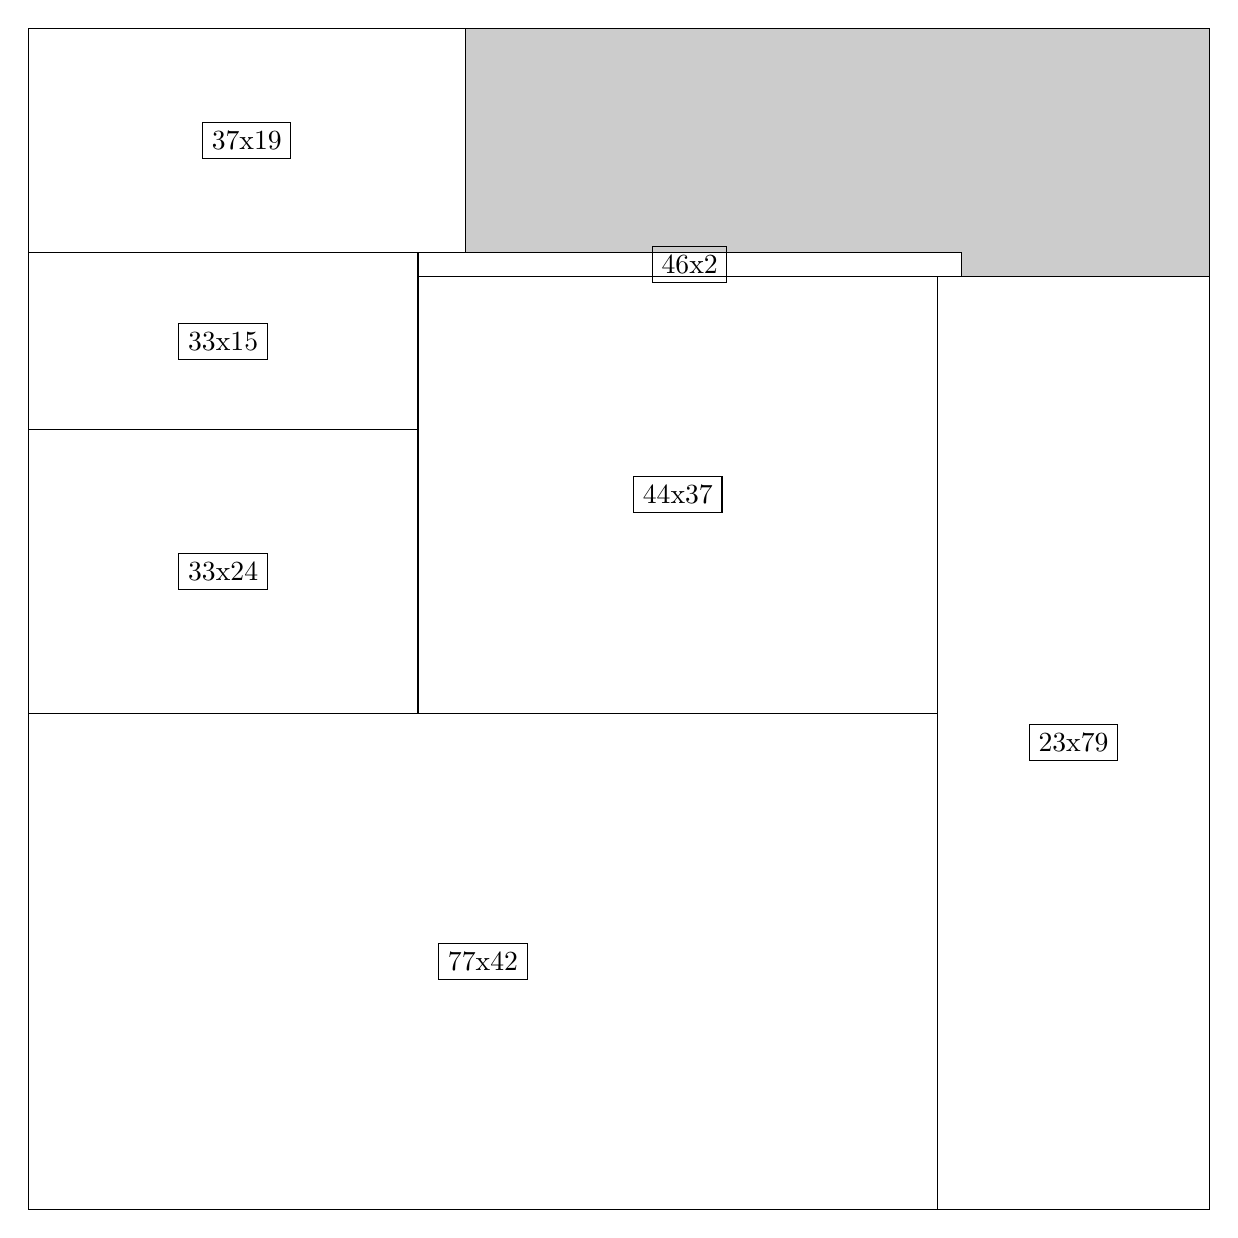
\begin{tikzpicture}[shorten >=1pt,scale=1.0,every node/.style={scale=1.0},->]
\tikzstyle{vertex}=[circle,fill=black!25,minimum size=14pt,inner sep=0pt]
\filldraw[fill=gray!40!white, draw=black] (0,0) rectangle (15.0,15.0);
\foreach \name/\x/\y/\w/\h in {77x42/0.0/0.0/11.549999999999999/6.3,23x79/11.549999999999999/0.0/3.4499999999999997/11.85,44x37/4.95/6.3/6.6/5.55,33x24/0.0/6.3/4.95/3.5999999999999996,37x19/0.0/12.15/5.55/2.85,33x15/0.0/9.9/4.95/2.25,46x2/4.95/11.85/6.8999999999999995/0.3}
\filldraw[fill=white!40!white, draw=black] (\x,\y) rectangle node[draw] (\name) {\name} ++(\w,\h);
\end{tikzpicture}


w =77 , h =42 , x =0 , y =0 , v =3234
\par
w =23 , h =79 , x =77 , y =0 , v =1817
\par
w =44 , h =37 , x =33 , y =42 , v =1628
\par
w =33 , h =24 , x =0 , y =42 , v =792
\par
w =37 , h =19 , x =0 , y =81 , v =703
\par
w =33 , h =15 , x =0 , y =66 , v =495
\par
w =46 , h =2 , x =33 , y =79 , v =92
\par
\newpage


\end{document}